% P1: Design and Evaluation of a Drift-Aware Continuous Learning MLOps Framework for Financial Transaction Fraud Detection
% Generated by build_latex.py from content.py. Compiles on Overleaf with pdflatex.
% To use the official BRAC template instead, paste chapters/*.tex and the bibliography there.
\documentclass[12pt,a4paper]{report}
\usepackage[margin=1in]{geometry}
\usepackage[T1]{fontenc}
\usepackage{graphicx,longtable,booktabs,array,enumitem,setspace}
\usepackage[hidelinks]{hyperref}
\usepackage{url}
\onehalfspacing
\setlist[enumerate]{itemsep=2pt}

\begin{document}
\pagenumbering{gobble}
\begin{titlepage}
\centering
{\LARGE\bfseries Design and Evaluation of a Drift-Aware Continuous Learning MLOps Framework for Financial Transaction Fraud Detection\par}
\vspace{1.5em} by\par\vspace{1em}
Mashud Hasan\\ 22299053\\[0.4em]
Nirnoy Biswas\\ 24241185\\[0.4em]
Md. Sabbir Hossain\\ 22299038\\[0.4em]
Al Imran\\ 231011035\\[0.4em]
Imtiaz Zaman Sami\\ 23101551\par
\vfill
A thesis submitted to the Department of Computer Science and Engineering\\ in partial fulfillment of the requirements for the degree of\\ B.Sc. in Computer Science and Engineering\par
\vspace{1.5em}
Department of Computer Science and Engineering\\ Brac University\\ [Month Year]\par
\vfill
\copyright 2026. Brac University\\ All rights reserved.
\end{titlepage}

\pagenumbering{roman}
\chapter*{Declaration}\addcontentsline{toc}{chapter}{Declaration}
It is hereby declared that
\begin{enumerate}
  \item The thesis submitted is our own original work while completing degree at Brac University.
  \item The thesis does not contain material previously published or written by a third party, except where this is appropriately cited through full and accurate referencing.
  \item The thesis does not contain material which has been accepted, or submitted, for any other degree or diploma at a university or other institution.
  \item We have acknowledged all main sources of help.
\end{enumerate}
\vspace{1em}\noindent\textbf{Student's Full Name \& Signature:}\par
\begin{minipage}[t]{0.45\textwidth}\centering\vspace{2.2em}\rule{0.8\textwidth}{0.4pt}\\ Mashud Hasan\\ 22299053\end{minipage}
\hfill
\begin{minipage}[t]{0.45\textwidth}\centering\vspace{2.2em}\rule{0.8\textwidth}{0.4pt}\\ Nirnoy Biswas\\ 24241185\end{minipage}
\hfill
\begin{minipage}[t]{0.45\textwidth}\centering\vspace{2.2em}\rule{0.8\textwidth}{0.4pt}\\ Md. Sabbir Hossain\\ 22299038\end{minipage}
\hfill
\begin{minipage}[t]{0.45\textwidth}\centering\vspace{2.2em}\rule{0.8\textwidth}{0.4pt}\\ Al Imran\\ 231011035\end{minipage}
\hfill
\begin{minipage}[t]{0.45\textwidth}\centering\vspace{2.2em}\rule{0.8\textwidth}{0.4pt}\\ Imtiaz Zaman Sami\\ 23101551\end{minipage}

\chapter*{Approval}\addcontentsline{toc}{chapter}{Approval}
The thesis titled ``Design and Evaluation of a Drift-Aware Continuous Learning MLOps Framework for Financial Transaction Fraud Detection'' submitted by
\begin{enumerate}
  \item Mashud Hasan (22299053)
  \item Nirnoy Biswas (24241185)
  \item Md. Sabbir Hossain (22299038)
  \item Al Imran (231011035)
  \item Imtiaz Zaman Sami (23101551)
\end{enumerate}
of Spring, 2026 has been accepted as satisfactory in partial fulfillment of the requirement for the degree of B.Sc. in Computer Science and Engineering in Summer 2026.

\vspace{1em}\noindent\textbf{Examining Committee:}\par\vspace{0.5em}
\noindent\begin{minipage}[t]{0.3\textwidth}\textbf{Supervisor:}\\ (Member)\end{minipage}\begin{minipage}[t]{0.65\textwidth}\vspace{1.5em}\rule{0.7\textwidth}{0.4pt}\\ Md. Sabbir Ahmed\\ Senior Lecturer\\ Department of Computer Science and Engineering\\ Brac University\end{minipage}\\[1.5em]
\noindent\begin{minipage}[t]{0.3\textwidth}\textbf{Co-Supervisor:}\\ (Member)\end{minipage}\begin{minipage}[t]{0.65\textwidth}\vspace{1.5em}\rule{0.7\textwidth}{0.4pt}\\ Naima Tahsin Nodi\\ Adjunct Lecturer\\ Department of Computer Science and Engineering\\ Brac University\end{minipage}\\[1.5em]
\noindent\begin{minipage}[t]{0.3\textwidth}\textbf{Thesis Coordinator:}\\ (Member)\end{minipage}\begin{minipage}[t]{0.65\textwidth}\vspace{1.5em}\rule{0.7\textwidth}{0.4pt}\\ Dr. Md. Golam Rabiul Alam\\ Professor\\ Department of Computer Science and Engineering\\ Brac University\end{minipage}\\[1.5em]
\noindent\begin{minipage}[t]{0.3\textwidth}\textbf{Head of Department:}\\ (Chair)\end{minipage}\begin{minipage}[t]{0.65\textwidth}\vspace{1.5em}\rule{0.7\textwidth}{0.4pt}\\ Dr. Sadia Hamid Kazi\\ Chairperson\\ Department of Computer Science and Engineering\\ Brac University\end{minipage}\\[1.5em]

\chapter*{Abstract}\addcontentsline{toc}{chapter}{Abstract}
Machine-learning models for financial transaction fraud detection are usually trained once and evaluated on a random split of historical data. In production, this picture breaks down in three ways. Fraud patterns and customer behaviour change over time (concept drift), so a model that scores well at deployment gradually loses accuracy. The true label of a transaction only becomes known weeks later, when a chargeback is filed or the dispute window closes (label delay), so the system cannot see its own mistakes in time. And the tools that Machine Learning Operations (MLOps) platforms offer to decide when to retrain, mostly statistical drift detectors on the input data, have rarely been tested against these conditions in fraud detection.

The purpose of this thesis is to build a drift-aware MLOps framework for financial fraud detection that can identify when a deployed model is becoming outdated, decide when retraining is actually necessary, and safely deploy a better retrained model without unnecessary retraining. The framework monitors a deployed LightGBM model on delayed labels, retrains it on a sliding window of recent data, and promotes a new model only after a promotion gate confirms that it is at least as good as the live model on data neither has seen. It is built with MLflow for experiment tracking and model versioning, a FastAPI scoring service and a monitoring dashboard, and is evaluated by replaying the IEEE-CIS Fraud Detection dataset (590,540 transactions over 182 days) as a live stream, with the Sparkov credit-card dataset (1.8 million transactions over two years) as a replication. Retraining strategies are compared under label delays of 0 to 60 days using time-ordered evaluation, paired day-block bootstrap confidence intervals, walk-forward tuning and repeated training seeds.

Preliminary results on IEEE-CIS show that weekly PR-AUC of a model trained once fell from 0.61 to 0.39 while the drift of its scores stayed far below the usual alarm level, that the benefit of retraining shrinks from +0.078 to +0.010 PR-AUC as labels arrive later, and that a fixed retraining schedule on recent data outperformed a tuned drift-triggered policy at every label delay. In fault-injection tests, the promotion gate blocked every model trained on corrupted data. The study therefore argues that a drift-aware fraud system should be designed around what drift detection can and cannot observe under label delay.

\noindent\textbf{Keywords:} Financial fraud detection, concept drift, label delay, continuous learning, MLOps, model retraining, promotion gate, LightGBM, PR-AUC, IEEE-CIS

\chapter*{Acknowledgement}\addcontentsline{toc}{chapter}{Acknowledgement}
Firstly, we thank Allah, the Most High, for everything He has bestowed upon us.

We would like to express our sincere gratitude to our supervisor, Md. Sabbir Ahmed sir, and our co-supervisor, Naima Tahsin Nodi ma'am, for their guidance and support throughout this research. Their feedback helped us to sharpen the research question and to overcome the difficulties we faced during the work.

We also thank the IEEE Computational Intelligence Society and Vesta Corporation for releasing the IEEE-CIS Fraud Detection dataset, the maintainers of the Sparkov credit-card dataset, and all the researchers whose articles and open-source tools have shaped this work.

\tableofcontents
\listoffigures\addcontentsline{toc}{chapter}{List of Figures}
\listoftables\addcontentsline{toc}{chapter}{List of Tables}
\chapter*{Nomenclature}\addcontentsline{toc}{chapter}{Nomenclature}
The next list describes several symbols and abbreviations that will be used later within the body of the document.\par\vspace{0.5em}
\noindent\begin{tabular}{@{}p{0.18\textwidth}p{0.75\textwidth}@{}}
\textbf{ADWIN} & Adaptive Windowing (drift detector) \\
\textbf{API} & Application Programming Interface \\
\textbf{CI} & Confidence Interval \\
\textbf{DDM} & Drift Detection Method \\
\textbf{FDS} & Fraud Detection System \\
\textbf{GNN} & Graph Neural Network \\
\textbf{KS} & Kolmogorov-Smirnov (test) \\
\textbf{MLOps} & Machine Learning Operations \\
\textbf{PR-AUC} & Area Under the Precision-Recall Curve \\
\textbf{PSI} & Population Stability Index \\
\textbf{ROC-AUC} & Area Under the Receiver Operating Characteristic Curve \\
\textbf{SHAP} & SHapley Additive exPlanations \\
\textbf{SMOTE} & Synthetic Minority Over-sampling Technique \\
\end{tabular}

\clearpage
\pagenumbering{arabic}
\chapter{Introduction}

\section{Background}

Digital payments have become the default way of paying for goods and services. Card payments, online shopping, mobile banking and cross-border e-commerce now generate millions of transactions every day, and each of them is an opportunity for fraud. Financial crime is estimated to cost U.S. institutions alone more than 32 billion dollars each year \cite{uddin2026}. For banks and payment processors, detecting fraudulent transactions quickly and accurately is therefore both a financial and a trust problem.

Modern fraud detection systems (FDS) combine fixed business rules with machine-learning models that score each transaction and raise alerts for investigators \cite{dalpozzolo2018,alessi2026}. A large body of work has compared classifiers, ensembles and class-imbalance techniques on public data \cite{dang2021,abdelnaby2023,sohony2018,mienye2023}, and gradient boosted trees such as XGBoost have proved to be strong models for tabular fraud data \cite{amekoe2024,uddin2026}. Most of this work, however, studies the model at a single point in time: it is trained on a random sample of historical transactions and tested on another random sample from the same period.

Real systems do not work like that. A model is trained on the past and then used on the future, and the future does not stand still. Customers change their spending habits, merchants and products change, and fraudsters adapt their strategies to whatever the current model does not catch. This change in the relationship between transactions and fraud over time is known as concept drift \cite{pulicharla2019,kodakandla2024}. Under concept drift, a model that performed well at deployment slowly, and sometimes suddenly, becomes less accurate. Menezes and Filho, for example, found that the F1-score of graph neural network fraud detectors trained on the IEEE-CIS dataset fell by up to 40\% over the following weeks \cite{menezes2025}.

Fraud detection adds a second difficulty that most drift research does not consider: the true label of a transaction is not known when the model makes its decision. A fraud is usually confirmed only when the cardholder notices it and files a chargeback, and a legitimate transaction is only confirmed when the dispute window has passed. Dal Pozzolo et al. call this verification latency and show that it strongly affects how a fraud model can be updated \cite{dalpozzolo2018}, and Amekoe et al. showed that it changes which learning strategies work best \cite{amekoe2024}. In practice, the labels a system can learn from are often weeks old, which means that it can only notice that its performance has dropped long after the drop has happened.

Machine Learning Operations (MLOps) has emerged to handle exactly this kind of problem: keeping machine-learning models reliable after deployment through automated pipelines for training, versioning, monitoring and redeployment \cite{pulicharla2019,kodakandla2024}. A central MLOps practice is continuous training, where models are retrained either on a fixed schedule or when a monitoring signal indicates that the data has drifted \cite{pulicharla2019}. Recent research increasingly favours the second option, triggering retraining when statistical drift measures such as the Population Stability Index (PSI) or the Kolmogorov-Smirnov (KS) test exceed a threshold \cite{shakil2025,wong2025}. Whether such triggers actually track the performance of a fraud model when labels arrive late is, however, an open question. This thesis addresses that question and builds a framework around the answer.

\section{Rationale of the Study or Motivation}

The first motivation for this study is the gap between how fraud models are evaluated in research and how they are used in practice. Many studies report near-perfect results on public credit-card datasets using random train-test splits and synthetic oversampling \cite{mienye2023}. Dang et al. showed that such results can be inflated when resampling is applied before splitting \cite{dang2021}, and a random split has a similar effect in time: the model is tested on transactions from the same period it was trained on, so concept drift is invisible. A fraud model that will be deployed on future transactions must be evaluated on future transactions.

The second motivation is that the decision of when to retrain a model is costly in both directions. Retraining too rarely leaves a degraded model in service and lets fraud through. Retraining too often wastes computing resources and, more importantly, increases the chance of deploying a bad model, for example one trained on incomplete or corrupted data. MLOps systems therefore need a policy that decides when retraining is actually necessary and a safeguard that decides whether a newly trained model may replace the one in service.

The third motivation is that recent work proposing drift-triggered retraining has been evaluated under conditions that favour it. Shakil et al. proposed a feature-drift indicator to decide when retraining is warranted, but tested it on drift that was artificially induced into non-fraud datasets \cite{shakil2025}. Wong and Perumal reported that an agentic, drift-triggered retraining scheduler outperformed weekly retraining, but on a single industrial dataset with injected drift \cite{wong2025}. Yelleti retrained fraud models only when a drift detector fired, but assumed that labels arrive immediately \cite{yelleti2025}. Shakil et al. themselves note that statistical drift does not always correspond to a change in model performance \cite{shakil2025}.

Finally, we are motivated by our own preliminary experiments on the IEEE-CIS dataset, which already challenge the common assumption. A LightGBM model trained once lost about a third of its weekly PR-AUC over the following months, yet the drift of its prediction scores stayed far below the usual alarm level, and only one of its ten most important features drifted noticeably. On a second dataset, Sparkov, we observed the opposite: strong input drift with almost no loss of accuracy. If drift detectors can both miss real decay and raise false alarms, a drift-aware system has to be designed around what drift detection can and cannot see. This is the perspective this thesis takes.

\section{Problem Statement}

We consider a fraud detection model deployed on a continuous stream of card transactions. Each transaction must be scored immediately, but its fraud label becomes available only after a label delay of several days to several weeks. Over time the distribution of transactions and the relationship between transaction features and fraud change. The operator of the system must decide, at regular intervals, whether to retrain the model, which data to retrain it on, and whether the retrained model is safe to put into service.

Existing approaches leave several parts of this problem unresolved:

\begin{enumerate}
  \item \textbf{Unrealistic evaluation.} Most fraud studies use random splits of static data, so they cannot show how performance evolves after deployment or how much retraining helps \cite{abdelnaby2023,mienye2023}.
  \item \textbf{Unverified retraining triggers.} Label-free drift measures such as PSI and KS are widely used to trigger retraining, but whether they track the performance of a fraud model has not been established on real, naturally drifting data \cite{shakil2025,wong2025}.
  \item \textbf{Ignored label delay.} Most retraining studies assume that labels are available immediately, although verification latency is a defining property of fraud detection \cite{dalpozzolo2018,amekoe2024}.
  \item \textbf{No fair comparison of retraining policies.} Scheduled and drift-triggered retraining are rarely compared under the same conditions, with tuned settings, uncertainty estimates and realistic label delay.
  \item \textbf{Unsafe model updates.} Automated retraining can deploy a model trained on corrupted labels or features; few frameworks test whether their safeguards actually stop such models.
  \item \textbf{Limited reproducibility.} Studies with realistic operating conditions often rely on private bank data \cite{dalpozzolo2018,somasundaram2019,aldaoud2025}.
\end{enumerate}

This thesis addresses these gaps through the following research questions:

\begin{itemize}[label={}, leftmargin=2em]
  \item \textbf{RQ1:} How does the performance of a fraud detection model evolve after deployment, and do label-free drift measures reflect that change?
  \item \textbf{RQ2:} How much does retraining improve performance, and how does label delay change that benefit?
  \item \textbf{RQ3:} Does drift-triggered retraining outperform scheduled retraining when both are tuned fairly and evaluated with realistic label delay?
  \item \textbf{RQ4:} Can an MLOps framework built on these findings sustain performance on a live stream and prevent faulty models from reaching production?
\end{itemize}

\section{Objectives}

The aim of this research is to design and evaluate a drift-aware continuous learning MLOps framework for financial transaction fraud detection that can identify when a deployed model is becoming outdated, decide when retraining is actually necessary, and safely deploy a better retrained model without unnecessary retraining. The specific objectives are:

\begin{enumerate}
  \item To review existing research on fraud detection, concept drift, label delay, retraining strategies and MLOps, and identify the gaps this thesis addresses.
  \item To prepare two public fraud datasets, IEEE-CIS and Sparkov, for strictly time-ordered evaluation, without leakage from future transactions.
  \item To measure how a model trained once degrades over time, and whether label-free drift measures (PSI of features and of model scores) track that degradation.
  \item To simulate retraining strategies under label delays of 0 to 60 days: a static model, scheduled retraining on all past data or on a sliding window, and retraining triggered by drift in scores or by a drop in delayed-label performance.
  \item To compare these strategies with paired day-block bootstrap confidence intervals, walk-forward tuning of their settings and repeated training seeds.
  \item To implement an MLOps framework with delayed-label monitoring, a retraining policy, a promotion gate, a model registry, a scoring service and a monitoring dashboard.
  \item To test the safeguards of the framework by injecting realistic faults (corrupted labels, a chargeback outage and a feature unit bug) into its retraining jobs.
  \item To check whether the findings generalise by replicating the key experiments on the second dataset.
\end{enumerate}

\section{Methodology in Brief}

The study follows the workflow shown in Figure \ref{fig:method}. It begins with a review of the literature on fraud detection, concept drift and MLOps, which identifies the gaps listed in the problem statement. Two public datasets are then prepared. IEEE-CIS, released by the IEEE Computational Intelligence Society and Vesta Corporation, contains 590,540 real e-commerce transactions over 182 days with a fraud rate of 3.5\% and has been used in recent drift and fraud studies \cite{menezes2025,uddin2026}. Sparkov contains about 1.8 million simulated card transactions over two years with a fraud rate of 0.5\%. Both are sorted by time and used without any random shuffling; per-card behaviour features for Sparkov are computed only from each card's earlier transactions, so that no information from the future leaks into the model.

\begin{figure}[htbp]
  \centering
  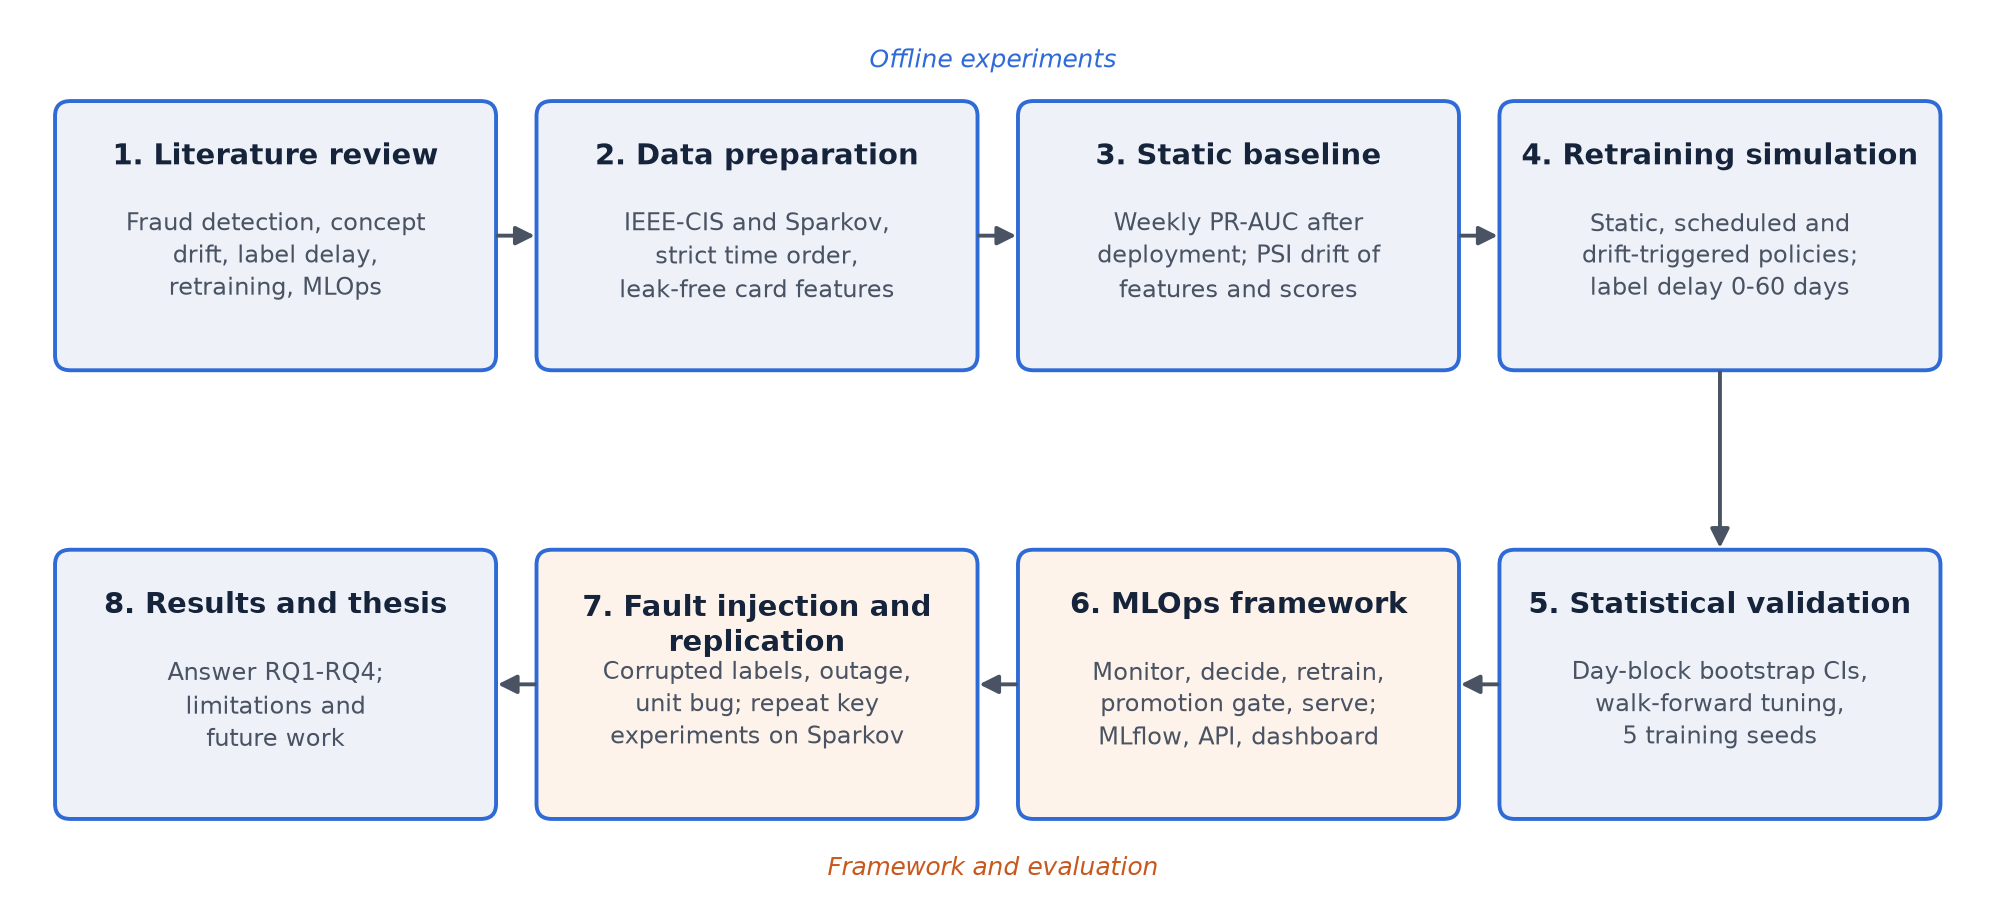
\includegraphics[width=\textwidth]{figures/methodology.png}
  \caption{Methodology of the study: from literature review and time-ordered data preparation to the retraining experiments, the framework and its evaluation}
  \label{fig:method}
\end{figure}

A LightGBM gradient boosted tree model is used throughout, because batch-trained boosted trees are strong, widely used models for tabular fraud data and remain competitive with incremental learners when labels are delayed \cite{amekoe2024}. The study first trains a static model and measures its weekly performance and the PSI drift of its features and scores over the following months. It then replays the later part of each dataset as a stream, week by week, and simulates the retraining strategies listed in the objectives, making labels available only after a chosen delay. PR-AUC is the main metric because fraud is rare and the precision of alerts matters most \cite{dalpozzolo2018}; results are averaged per week so that scores from different model versions are never pooled. Uncertainty is estimated with a paired bootstrap that resamples whole days, strategy settings are tuned walk-forward using only information available at the time, and the key comparisons are repeated with five training seeds.

The findings are then turned into a working framework, shown in Figure \ref{fig:loop}. Every week it measures the live model on labels that have become available, decides whether to retrain, trains a new model on a sliding window of recent labelled data, and promotes it only if a promotion gate confirms that it performs at least as well as the live model on data neither has seen. Models are versioned in MLflow, served through a FastAPI scoring service and tracked on a monitoring dashboard, following common MLOps practice \cite{pulicharla2019}. The framework is evaluated by replaying the stream end to end and by injecting faults into selected retraining jobs to test whether the promotion gate and performance safety net stop faulty models.

\begin{figure}[htbp]
  \centering
  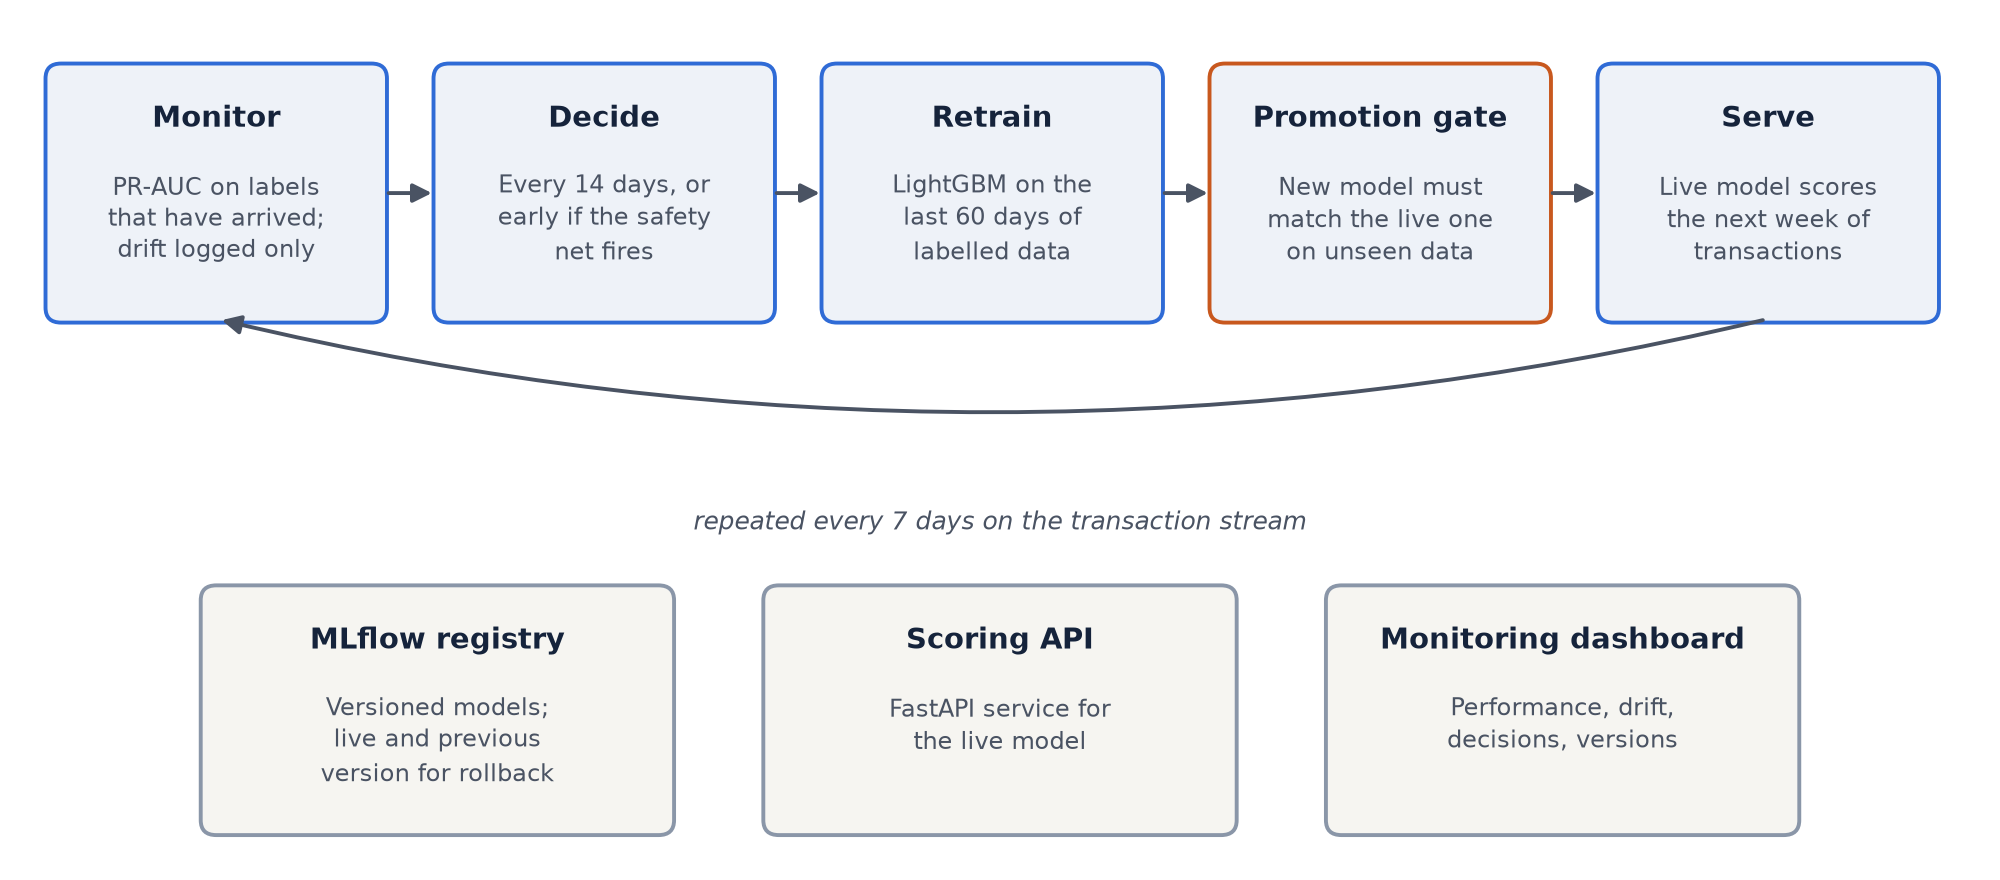
\includegraphics[width=\textwidth]{figures/framework_loop.png}
  \caption{The proposed continuous-learning loop, run every week on the transaction stream}
  \label{fig:loop}
\end{figure}

Preliminary experiments on IEEE-CIS have been completed. They show that a fixed schedule of retraining on the most recent 60 days outperformed a tuned drift-triggered policy at every label delay (by 0.03 to 0.07 PR-AUC), that the benefit of any retraining shrinks sharply when labels arrive 60 days late, and that the framework reproduces the offline results when replayed (0.531 mean weekly PR-AUC). The replication on Sparkov is in progress and will be reported together with the full results in later chapters.

\section{Scopes and Challenges}

The study focuses on binary fraud detection for card transactions, where each transaction is scored as fraudulent or legitimate. Its scope is the post-deployment life of a model: how it degrades, when retraining is actually necessary, and how model updates can be made safe. It does not aim to find the best possible classifier, and it does not connect to a real bank or process real customer data. The main areas covered are:

\begin{enumerate}
  \item Time-ordered evaluation of fraud models on two public datasets.
  \item Analysis of performance decay and of label-free drift measures after deployment.
  \item Comparison of static, scheduled and drift-triggered retraining under label delay.
  \item Statistical validation with bootstrap confidence intervals, walk-forward tuning and repeated seeds.
  \item An MLOps framework with monitoring, retraining policy, promotion gate, model registry, scoring service and dashboard.
  \item Fault-injection testing of the framework's safeguards.
\end{enumerate}

The study also faces several challenges:

\begin{enumerate}
  \item \textbf{Label delay:} performance can only be measured on labels that have matured, so problems are always detected late.
  \item \textbf{Class imbalance:} frauds are rare (0.5\% to 3.5\% of transactions), which makes weekly performance estimates noisy and requires careful statistics.
  \item \textbf{Simulated deployment:} the stream is replayed from historical data, so live latency and real label-feed behaviour are not observed.
  \item \textbf{Limited datasets:} public fraud data with timestamps is scarce; IEEE-CIS covers only six months and Sparkov is simulated.
  \item \textbf{Anonymised features:} many IEEE-CIS features are masked, which limits the interpretation of which features drift and why.
  \item \textbf{Computational cost:} repeated retraining over long streams, several label delays and many policy settings requires hours of computation per experiment.
  \item \textbf{Generalisation:} results obtained with one model family and two datasets may not transfer to every institution or fraud type.
\end{enumerate}

Despite these challenges, the study can provide practical, evidence-based guidance on how fraud detection models should be maintained after deployment, and a reproducible open framework that implements it.

\chapter{Literature Review}

\section{Preliminaries}

\textbf{Fraud detection as a learning problem.} Transaction fraud detection is a binary classification task on a continuous stream of transactions. Frauds are rare, typically well under 5\% of transactions, so the task is highly imbalanced and accuracy is a misleading measure \cite{abdelnaby2023,aldaoud2025}. Precision and recall of the fraud class, and summary measures such as PR-AUC, describe performance more faithfully. In an operational FDS, investigators can only check a limited number of alerts per day, so the precision of the top-ranked alerts matters most \cite{dalpozzolo2018}.

\textbf{Concept drift.} Model drift is the loss of performance that follows when deployed data no longer resembles the training data \cite{pulicharla2019}. It takes several forms: \textit{concept drift}, where the relationship between features and labels changes; \textit{covariate shift}, where the distribution of the input features changes; and \textit{label drift}, where the frequency of the classes changes \cite{pulicharla2019,kodakandla2024}. Only a change in the relationship between features and labels necessarily harms a model; a change in the inputs may or may not. Drift can also be described by how it unfolds, as illustrated in Figure \ref{fig:drift}. In \textit{sudden} drift the old pattern is replaced at once; in \textit{gradual} drift the old and new patterns alternate, with the new one becoming more frequent; in \textit{incremental} drift the pattern moves slowly through intermediate states; and in \textit{recurring} drift earlier patterns return, for example with seasonal spending. Fraud is an adversarial setting, so drift is frequent, irregular and partly caused by the detection system itself \cite{menezes2025,hassan2026}.

\begin{figure}[htbp]
  \centering
  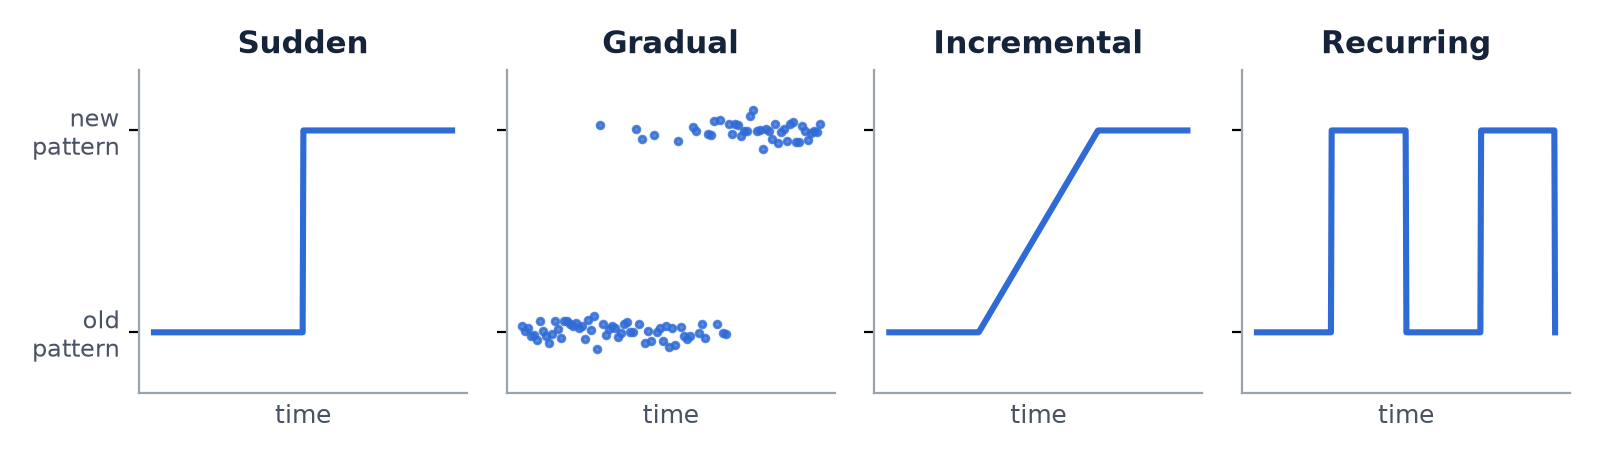
\includegraphics[width=\textwidth]{figures/drift_types.png}
  \caption{Types of concept drift by how the underlying fraud pattern changes over time}
  \label{fig:drift}
\end{figure}

\textbf{Drift detection.} Drift detectors fall into two broad groups. Label-free detectors compare the distribution of recent inputs or model scores with a reference, using measures such as the PSI, the KS test or the Kullback-Leibler divergence \cite{shakil2025,wong2025}; they can run immediately but only see changes in the inputs or the scores. The PSI is commonly read as stable below 0.1, moderately shifted between 0.1 and 0.25, and strongly shifted above 0.25, and Wong and Perumal used 0.25 as their retraining threshold \cite{wong2025}. Error-based detectors such as DDM, EDDM and ADWIN monitor the model's error rate and signal drift when it rises \cite{yelleti2025,aldaoud2025}; they detect real drift but need labels, which in fraud detection arrive late.

\textbf{Verification latency.} In a real FDS, most transactions are labelled only after a delay, when a fraud is reported or when the dispute period ends. A small number of alerted transactions receive quick feedback from investigators. Dal Pozzolo et al. formalised this as verification latency and the alert-feedback interaction, and showed that it changes which data a model can learn from and when \cite{dalpozzolo2018}. Figure \ref{fig:delay} shows the consequence for an automated system. At any moment, the most recent weeks of transactions have already been scored but not yet labelled. Performance can therefore only be measured on older, matured transactions, and a retrained model can only learn from data that ends one label delay before the present. The longer the delay, the later a performance drop is noticed and the older the data a new model is trained on.

\begin{figure}[htbp]
  \centering
  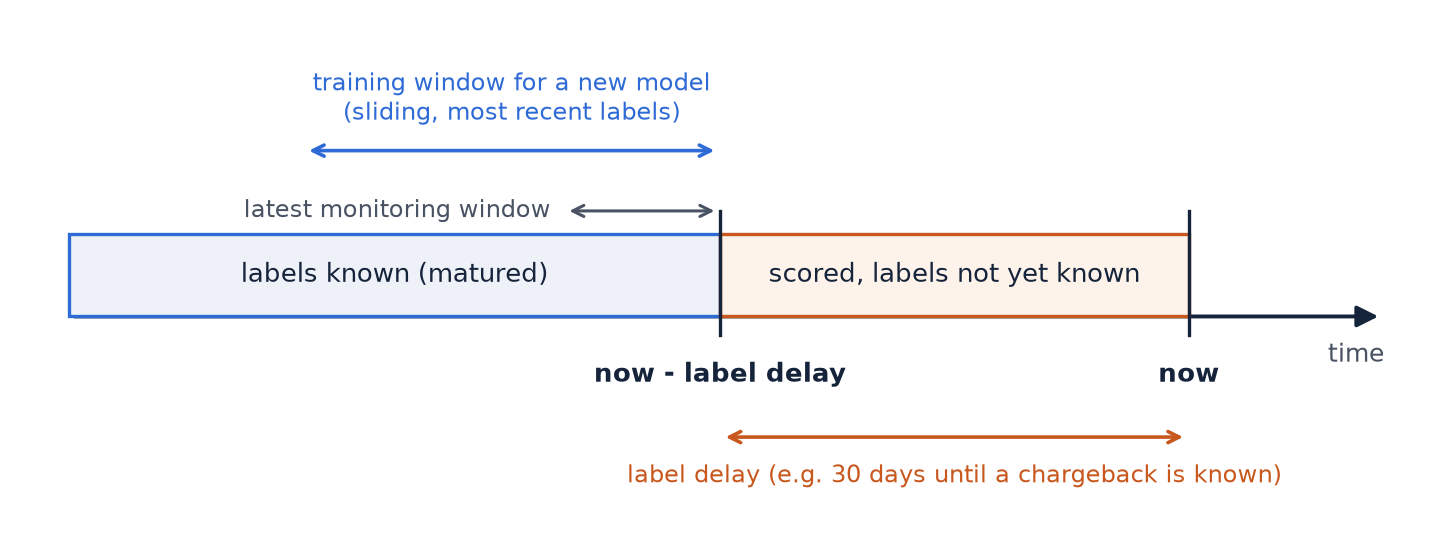
\includegraphics[width=\textwidth]{figures/label_delay.png}
  \caption{Label delay in a fraud detection system: transactions are scored immediately, but their labels become usable only after the delay, which limits both monitoring and retraining}
  \label{fig:delay}
\end{figure}

\textbf{Adaptation strategies.} A deployed model can be kept up to date in several ways. \textit{Periodic} or scheduled retraining rebuilds the model at fixed intervals, while \textit{event-driven} or triggered retraining rebuilds it when a monitoring signal crosses a threshold \cite{pulicharla2019}. The training data may be all history (an expanding window) or only recent data (a sliding window), which forgets outdated patterns \cite{dalpozzolo2018}. \textit{Incremental} or online learning updates the model with every new labelled transaction, and \textit{ensemble} methods combine models trained on different periods \cite{somasundaram2019,yelleti2025}. Which of these works best depends on how quickly labels arrive: under label delay, batch learning can match or beat instance-incremental learning \cite{amekoe2024}.

\textbf{MLOps.} MLOps applies software-engineering practice to the machine-learning lifecycle: automated training pipelines, experiment tracking, versioned model registries, continuous integration and delivery, and monitoring in production \cite{pulicharla2019,kodakandla2024}. Tools such as MLflow, Kubeflow and Apache Airflow automate retraining, while Prometheus, Grafana and Evidently AI support monitoring \cite{pulicharla2019}. Recent MLOps frameworks close the loop between monitoring and retraining for specific domains, such as phishing detection \cite{reda2025} and industrial prediction \cite{wong2025}. A common deployment pattern keeps the model in service (the champion) and promotes a newly trained candidate (the challenger) only if it passes an evaluation, which is the idea behind the promotion gate used in this thesis.

\textbf{Explainability under drift.} Financial regulators expect model decisions to be transparent and auditable, so fraud and credit models are increasingly paired with explanation methods such as SHAP \cite{uddin2026,alessi2026}. Drift affects these explanations too: explanations computed against an outdated reference population can become unstable or unfair as the population changes \cite{john2025}.

\textbf{Evaluation over time.} Evaluating a drifting system requires respecting time: models may only be trained on data from before the period they are tested on \cite{menezes2025}. Common designs include a single chronological split, rolling or walk-forward evaluation, and replaying a historical stream. Because consecutive transactions are correlated, uncertainty estimates should resample whole blocks of time rather than individual transactions.

\section{Review of Existing Research}

\textbf{Fraud detection under drift and label delay.} Dal Pozzolo et al. \cite{dalpozzolo2018} provided one of the most realistic models of a credit-card fraud detection system. Working with an industrial partner and more than 75 million e-commerce transactions collected over three years, they described the layers of an FDS, from terminal checks and blocking rules to the data-driven model and human investigators. They formalised verification latency and the alert-feedback interaction, argued that alert precision is the most meaningful performance measure, and proposed training separate classifiers on recent investigator feedback and on delayed labels, then aggregating their outputs. Their experiments showed that giving more weight to recent feedback produced more precise alerts, and that sliding-window and ensemble approaches handled drift. The work is the foundation for treating label delay as a first-class concern. Its limitations for this thesis are that the data is private, that the timing of retraining is not studied, and that the model is not embedded in an MLOps workflow with monitoring and safe deployment.

Amekoe et al. \cite{amekoe2024} compared instance-incremental learning with batch learning for fraud detection when labels arrive with a delay. Instance-incremental algorithms are usually preferred for evolving streams, but they assume that each label is available immediately. Using fraud detection data and generated datasets, the authors found that instance-incremental learning, including the Adaptive Random Forest, was not the superior option compared with batch-trained models such as XGBoost, and that batch solutions are also easier to interpret. This finding directly supports the design choice of this thesis to retrain a batch model on windows of delayed labels. The study compares learning paradigms, however, and does not examine when to retrain or how to deploy a new model safely.

Yelleti \cite{yelleti2025} proposed ROSFD, a two-stage framework for online streaming fraud detection. An initial model is built offline with incremental learning to avoid a cold start, and in production the drift detectors DDM, EDDM and ADWIN decide when the model is retrained incrementally. Across five datasets, ADWIN gave the best results among the detectors and the Adaptive Random Forest achieved the highest AUC on four of them, while the train-only-when-required strategy substantially reduced how often the model was retrained without a large loss of AUC. The study is close to the question of this thesis, since it tests retraining only when needed. It reports ROC-AUC, which is less informative than PR-AUC for rare fraud, and it assumes labels are available immediately, which makes error-based detectors look more responsive than they would be in practice.

Somasundaram and Reddy \cite{somasundaram2019} proposed a parallel and incremental fraud detection model, Transaction Window Bagging, which combines parallel bagging, incremental learning, cost-sensitive learning and weighted voting to handle concept drift and class imbalance together. Evaluated on Brazilian bank data, it improved the fraud detection rate and the misclassification cost compared with other models. The study is valuable because it treats fraud detection as a continuous stream rather than a static dataset. However, the data is private, label delay is not modelled, and the effect of retraining frequency is not isolated.

Al-Daoud and Abu-AlSondos \cite{aldaoud2025} proposed a hybrid machine-learning framework for fraud detection in Gulf Cooperation Council banks that addresses class imbalance (SMOTEBoost and cost-sensitive learning), adversarial attacks (adversarial training and a FraudGAN), concept drift (DDM and ADWIN) and explainability (SHAP, LIME and human-in-the-loop review). On real bank transactions, the framework raised fraud recall from 35\% to 85\%, reduced the success rate of adversarial attacks from 35\% to 5\%, and recovered from drift within 24 hours while keeping latency below 150 milliseconds. The study shows that drift handling must work together with the other demands of a production fraud system. Drift, however, is one component among many, the retraining policy is not compared with alternatives, and the private data prevents replication.

Alessi and Fugini \cite{alessi2026} developed a real-time financial fraud detection system for transaction data streams that addresses extreme class imbalance and concept drift. It uses a lightweight data stream management system for real-time feature engineering, combines deterministic rules with adaptive machine-learning models, manages the decision threshold dynamically to balance precision and recall, and compares several adaptive learning strategies. It also introduces an interpretability framework that turns low-level feature attributions into concepts investigators can act on. The work demonstrates a practical, operational view of adaptive fraud detection, but it does not test safeguards against faulty model updates or evaluate the effect of label delay on the retraining decision.

Menezes and Filho \cite{menezes2025} studied how graph neural network fraud detectors degrade under natural data drift. They built a heterogeneous knowledge graph from 284,000 IEEE-CIS transactions, trained R-GCN, HGT and HAN models on the earliest 70\%, and then froze the models and monitored them over 50 subsequent 12-hour windows. All models degraded in a volatile, non-monotonic way; the F1-score of HGT fell from 0.747 to as low as 0.455, while the simpler R-GCN was the most stable. They also observed that AUC stayed stable while F1 fluctuated, suggesting that score distributions shift and fixed decision thresholds become outdated. The study is directly relevant because it uses the same dataset and confirms that drift is a real problem on it. However, it only measures degradation: no retraining strategy is evaluated, label delay is not modelled, and the proposed mitigation framework is conceptual.

Hassan \cite{hassan2026} proposed DriftGuard-TriAudit, a concept-drift-aware continual learning framework for financial statement fraud that jointly analyses financial ratios, management discussion text and document layout. It adds modality-specific drift monitoring, reliability-weighted fusion of the three modalities, and memory-based continual learning. On a synthetic benchmark with four temporal fraud scenarios, it achieved an average precision of 0.628 and improved precision over standard continual fine-tuning (0.547 against 0.428) with a similar AUC. The work shows that drift-aware continual learning is relevant beyond transaction fraud, but it concerns a different kind of fraud and is evaluated only on synthetic data.

\textbf{Retraining decisions and MLOps.} Shakil et al. \cite{shakil2025} proposed a feature-drift-guided retraining framework for MLOps. They combined the KS statistic with a confidence-based model performance indicator and a new feature-level indicator, the percent mean shift, and retrained a model only when all three signalled drift and enough drifted data was available. Using simulated mean and variance shifts on health, loan-approval and benchmark datasets with Random Forest and SVM models, they showed that the percent mean shift correlated with performance loss more strongly than the KS statistic alone, and that the framework matched existing drift detectors while retraining less often. The study addresses exactly the question of when retraining is warranted. Its drift is artificially induced into one feature at a time, however, the datasets are not fraud streams, label delay is ignored, and the confidence-based indicator does not measure whether predictions are correct.

Wong and Perumal \cite{wong2025} proposed an AI-driven model-retraining architecture that combines drift detection (the KS test and ADWIN, with PSI and Kullback-Leibler divergence to measure severity), an agentic orchestrator that schedules retraining using a reinforcement-learning policy, and data-governance controls with a composite data-quality index. In a smart-manufacturing case study with injected sensor drift, the architecture raised the F1-score from 0.62 after drift to 0.93, and outperformed a weekly retraining schedule while retraining only three times in six months. Its strengths are the integration of retraining with data quality and the explicit comparison with scheduled retraining. The evidence is, however, limited to one dataset with artificially controlled drift, reported without confidence intervals or repeated runs, and labels are assumed to be available immediately. The comparison with scheduled retraining is therefore an important claim that this thesis re-examines on real fraud data with label delay.

Reda et al. \cite{reda2025} presented HAMF, a hybrid MLOps framework that manages the whole lifecycle of adaptive phishing detection models. Its microservices architecture links data ingestion, SHAP-guided feature replacement, event-driven retraining, monitoring, fairness auditing and stakeholder feedback in a closed loop of 13 pipeline stages. On three phishing datasets, it detected drift within 18 seconds, recovered an F1-score above 0.99 after drift, reduced fairness disparity by 60\%, and handled 2,300 requests per second with a p99 latency below 50 milliseconds, outperforming SageMaker and Kubeflow with MLflow baselines. HAMF is a strong example of a complete, closed-loop MLOps framework. Phishing detection, however, receives labels far faster than card fraud, so its event-driven design cannot be transferred directly to a setting with weeks of label delay.

Kodakandla \cite{kodakandla2024} described an end-to-end MLOps approach for detecting and mitigating data drift in real-time systems across healthcare, finance and the Internet of Things, combining automated drift detection, retraining techniques and adaptive models with attention to governance and ethics. Pulicharla \cite{pulicharla2019} reviewed methods for detecting model drift and automating retraining in ML pipelines, covering statistical tests, drift detection algorithms, monitoring tools and retraining pipelines, and discussed the trade-off between scheduled and event-driven retraining. These works describe what an MLOps system for drifting data should contain, but they are conceptual and do not measure which retraining policy works best for fraud detection under label delay.

Kaushik et al. \cite{kaushik2025} proposed an architecture for real-time analytics that embeds machine-learning detection into streaming data pipelines built on Kafka and Flink. It includes a feedback-driven module for online model updates, adaptive stream operators, hybrid edge-cloud execution and a self-healing pipeline. In simulation, an adaptive random forest with feedback achieved higher detection accuracy and a lower false-positive rate than static Isolation Forest and k-NN detectors, with lower latency. The paper usefully places fraud detection within a production data architecture. Its evaluation is based on simulated workloads and synthetic data, so its results cannot show how such a system behaves on real fraud streams or under label delay.

\textbf{Explainability under drift.} Uddin and Aziz \cite{uddin2026} proposed a SHAP-guided adaptive ensemble for explainable financial fraud detection and checked it against U.S. regulatory requirements. Using the 590,540 transactions of IEEE-CIS, they found that XGBoost with TreeExplainer gave nearly perfectly stable explanations, while an LSTM's explanations were weak; the adaptive ensemble reached an AUC-ROC of 0.8837 on held-out data, and a GraphSAGE model reached 0.9248. John \cite{john2025} studied credit scoring under concept drift and showed that SHAP explanations computed against a fixed background become unstable and unfair as populations change; drift-aware rebaselining of the background and online surrogate calibration improved stability and reduced disparate impact without hurting accuracy. Together, these studies indicate that a model's explanations, not only its predictions, need maintenance under drift, which is a natural extension of the framework in this thesis.

\textbf{Static fraud classification.} A large group of studies focuses on maximising performance on a static dataset. Mienye and Sun \cite{mienye2023} proposed a deep-learning ensemble with LSTM and GRU base learners, a multilayer perceptron meta-learner and SMOTE-ENN resampling, and reported a sensitivity of 1.000 and a specificity of 0.997. Sohony et al. \cite{sohony2018} combined feed-forward neural networks and random forests in an ensemble to balance fraud recall against false alarms. Abd El-Naby et al. \cite{abdelnaby2023} combined balancing methods such as SMOTE, Borderline-SMOTE, ADASYN and SMOTETomek with classical classifiers and reported high accuracy after balancing. Dang et al. \cite{dang2021} compared resampling methods, classical models and deep reinforcement learning, and showed that resampling before the train-test split can make results look far better than they are. These studies establish strong classifiers and careful imbalance handling, but they use random splits of static data, so they do not show how the models would perform after deployment.

Table \ref{tab:review} summarises the studies most closely related to this thesis.

{\footnotesize
\begin{longtable}{>{\raggedright\arraybackslash}p{0.16\textwidth}>{\raggedright\arraybackslash}p{0.19\textwidth}>{\raggedright\arraybackslash}p{0.19\textwidth}>{\raggedright\arraybackslash}p{0.11\textwidth}>{\raggedright\arraybackslash}p{0.29\textwidth}}
\caption{Summary of the most closely related studies}\label{tab:review}\\
\toprule
\textbf{Study} & \textbf{Data} & \textbf{Drift handling} & \textbf{Label delay} & \textbf{Main limitation for this thesis} \\
\midrule
\endfirsthead
\toprule
\textbf{Study} & \textbf{Data} & \textbf{Drift handling} & \textbf{Label delay} & \textbf{Main limitation for this thesis} \\
\midrule
\endhead
Dal Pozzolo et al. \cite{dalpozzolo2018} & 75M+ real card transactions, 3 years & Sliding window and ensembles; separate feedback and delayed models & Yes (core) & Private data; retraining timing and MLOps integration not studied \\ \midrule
Amekoe et al. \cite{amekoe2024} & Fraud data and generated streams & Instance-incremental vs. batch learning & Yes (core) & No drift-triggered retraining or safe deployment \\ \midrule
Yelleti \cite{yelleti2025} & Five fraud datasets & DDM, EDDM, ADWIN trigger incremental retraining & No & Evaluated with ROC-AUC only; labels assumed immediate \\ \midrule
Al-Daoud and Abu-AlSondos \cite{aldaoud2025} & Private GCC bank transactions & DDM and ADWIN with adaptive learning & No & Private data; drift handled as one part of a larger framework \\ \midrule
Alessi and Fugini \cite{alessi2026} & Transaction data streams & Compares adaptive learning strategies; dynamic threshold & Not central & No promotion checks or fault testing \\ \midrule
Somasundaram and Reddy \cite{somasundaram2019} & Brazilian bank data & Transaction-window bagging, incremental & No & Private data; no label delay \\ \midrule
Menezes and Filho \cite{menezes2025} & IEEE-CIS (subset) as a graph & None: frozen models monitored & No & Measures decay only; no retraining evaluated \\ \midrule
Shakil et al. \cite{shakil2025} & Health, loan and benchmark datasets & KS + mean-shift indicator triggers retraining & No & Artificially induced drift; not fraud \\ \midrule
Wong and Perumal \cite{wong2025} & Manufacturing sensor data & PSI/KL + ADWIN, agentic retraining scheduler & No & Injected drift; single run; no confidence intervals \\ \midrule
Reda et al. \cite{reda2025} & Phishing URL datasets & Event-driven retraining in a closed-loop MLOps pipeline & No & Different domain; drift simulated \\ \midrule
Mienye and Sun \cite{mienye2023} & Public card datasets & None (static) & No & Random split with resampling; no temporal evaluation \\ \bottomrule
\end{longtable}
}

\section{Summary of Key Findings}

The literature agrees that concept drift is a real and serious problem for fraud detection. Static models degrade after deployment, sometimes sharply and irregularly \cite{menezes2025,dalpozzolo2018}, and fraud detection systems therefore need a way to update their models over time. Sliding windows, incremental learning, ensembles and drift-triggered retraining have all been proposed \cite{dalpozzolo2018,somasundaram2019,yelleti2025,aldaoud2025,alessi2026}.

Label delay is a defining feature of fraud detection but is rarely modelled. Dal Pozzolo et al. and Amekoe et al. showed its importance \cite{dalpozzolo2018,amekoe2024}, yet most retraining frameworks assume that labels are immediately available \cite{shakil2025,wong2025,yelleti2025,kaushik2025}. Because error-based drift detectors depend on labels, label delay directly limits how quickly any performance-based trigger can react.

Recent MLOps research favours retraining triggered by drift detection, and reports that it outperforms or matches scheduled retraining with fewer retrains \cite{shakil2025,wong2025,yelleti2025}. These claims rest on artificially induced drift, single datasets, non-fraud domains or immediate labels. At the same time, statistical drift does not always correspond to a loss of performance \cite{shakil2025}. Whether drift-triggered retraining is better for fraud detection under realistic conditions is therefore unresolved.

Evaluation practice is a further gap. Many fraud studies report very high results from random splits of static data \cite{mienye2023,abdelnaby2023}, which says little about performance after deployment. Few studies use time-ordered evaluation, confidence intervals, fair tuning of competing strategies or repeated runs, and studies with realistic streams often use private data that cannot be reproduced \cite{dalpozzolo2018,somasundaram2019,aldaoud2025}.

Safe deployment of retrained models also receives little attention. MLOps frameworks close the loop between monitoring and retraining \cite{reda2025,kodakandla2024}, and some compare a new model with the current one \cite{wong2025}, but we found no fraud detection study that tests whether such safeguards actually stop models trained on corrupted labels or features. Finally, drift also affects the stability of explanations \cite{john2025,uddin2026}, which matters for regulated financial systems.

Based on these findings, this thesis proposes a drift-aware continuous learning MLOps framework for financial transaction fraud detection that: (1) is evaluated on public data in strict time order, with confidence intervals, walk-forward tuning and repeated seeds; (2) models label delay explicitly and measures how it limits the benefit of retraining; (3) compares scheduled and drift-triggered retraining fairly and retrains only when the evidence shows it is necessary; (4) monitors performance on delayed labels rather than relying only on label-free drift signals; (5) protects production with a promotion gate and a performance safety net, tested by fault injection; and (6) is released as reproducible open-source code with a second dataset for replication. The following chapters describe the requirements, the methodology and the results of this framework in detail.


\clearpage
\addcontentsline{toc}{chapter}{Bibliography}
% IEEE style, numbered in order of first citation
\begin{thebibliography}{99}
\bibitem{uddin2026}
M. N. Uddin and M. M. Aziz, ``Shapley value-guided adaptive ensemble learning for explainable financial fraud detection with U.S. regulatory compliance validation,'' arXiv preprint arXiv:2604.14231, 2026.

\bibitem{dalpozzolo2018}
A. Dal Pozzolo, G. Boracchi, O. Caelen, C. Alippi, and G. Bontempi, ``Credit card fraud detection: A realistic modeling and a novel learning strategy,'' \textit{IEEE Transactions on Neural Networks and Learning Systems}, vol. 29, no. 8, pp. 3784--3797, 2018. doi: 10.1109/TNNLS.2017.2736643.

\bibitem{alessi2026}
G. Alessi and M. Fugini, ``Adaptive real-time financial fraud detection with explainable AI tools,'' \textit{Digital Threats: Research and Practice}, vol. 7, no. 1, pp. 1--31, 2026. doi: 10.1145/3794859.

\bibitem{dang2021}
T. Dang, T. Tran, L. Tuan, and M. Tiep, ``Machine learning based on resampling approaches and deep reinforcement learning for credit card fraud detection systems,'' \textit{Applied Sciences}, vol. 11, no. 21, p. 10004, 2021. doi: 10.3390/app112110004.

\bibitem{abdelnaby2023}
A. Abd El-Naby, E. E.-D. Hemdan, and A. El-Sayed, ``An efficient fraud detection framework with credit card imbalanced data in financial services,'' \textit{Multimedia Tools and Applications}, vol. 82, pp. 4139--4160, 2023. doi: 10.1007/s11042-022-13434-6.

\bibitem{sohony2018}
I. Sohony, R. Pratap, and U. Nambiar, ``Ensemble learning for credit card fraud detection,'' in \textit{Proceedings of the ACM India Joint International Conference on Data Science and Management of Data (CoDS-COMAD)}, 2018, pp. 289--294. doi: 10.1145/3152494.3156815.

\bibitem{mienye2023}
I. D. Mienye and Y. Sun, ``A deep learning ensemble with data resampling for credit card fraud detection,'' \textit{IEEE Access}, vol. 11, pp. 30628--30638, 2023. doi: 10.1109/ACCESS.2023.3262020.

\bibitem{amekoe2024}
K. M. Amekoe, M. Lebbah, G. Jaffre, H. Azzag, and Z. Chelly Dagdia, ``Evaluating the efficacy of instance incremental vs. batch learning in delayed label environments: An empirical study on tabular data streaming for fraud detection,'' arXiv preprint arXiv:2409.10111, 2024. doi: 10.48550/arXiv.2409.10111.

\bibitem{pulicharla2019}
M. R. Pulicharla, ``Detecting and addressing model drift: Automated monitoring and real-time retraining in ML pipelines,'' \textit{World Journal of Advanced Research and Reviews}, vol. 3, no. 2, pp. 147--152, 2019. doi: 10.30574/wjarr.2019.3.2.0189.

\bibitem{kodakandla2024}
N. Kodakandla, ``Data drift detection and mitigation: A comprehensive MLOps approach for real-time systems,'' \textit{International Journal of Science and Research Archive}, vol. 12, no. 1, pp. 3127--3139, 2024. doi: 10.30574/ijsra.2024.12.1.0724.

\bibitem{menezes2025}
R. S. Menezes and R. H. Filho, ``Semantic and structural drift in financial knowledge graphs: A robustness analysis of GNN-based fraud detectors,'' in \textit{2025 IEEE International Conference on Knowledge Graph (ICKG)}, Limassol, Cyprus, 2025, pp. 285--291. doi: 10.1109/ICKG66886.2025.00044.

\bibitem{shakil2025}
M. N. P. Shakil, M. S. Islam, N. Noman, and M. Papini, ``Feature drift-guided adaptive ML retraining: An MLOps approach for big data analytics,'' in \textit{2025 IEEE International Conference on Big Data (BigData)}, Macau, China, 2025, pp. 7719--7727. doi: 10.1109/BigData66926.2025.11401445.

\bibitem{wong2025}
H. M. Wong and S. Perumal, ``AI-driven model-retraining architecture to sustain operational accuracy in data-drifting environments,'' in \textit{2025 IEEE Symposium on Wireless Technology \& Applications (ISWTA)}, Penang, Malaysia, 2025, pp. 1--6. doi: 10.1109/ISWTA68114.2025.11329530.

\bibitem{yelleti2025}
V. Yelleti, ``ROSFD: Robust online streaming fraud detection with resilience to concept drift in data streams,'' arXiv preprint arXiv:2504.10229, 2025.

\bibitem{somasundaram2019}
A. Somasundaram and S. Reddy, ``Parallel and incremental credit card fraud detection model to handle concept drift and data imbalance,'' \textit{Neural Computing and Applications}, vol. 31, pp. 3--14, 2019. doi: 10.1007/s00521-018-3633-8.

\bibitem{aldaoud2025}
K. I. Al-Daoud and I. A. Abu-AlSondos, ``Robust AI for financial fraud detection in the GCC: A hybrid framework for imbalance, drift, and adversarial threats,'' \textit{Journal of Theoretical and Applied Electronic Commerce Research}, vol. 20, no. 2, p. 121, 2025. doi: 10.3390/jtaer20020121.

\bibitem{hassan2026}
Y. Hassan, ``DriftGuard-TriAudit: Concept-drift-aware continual multimodal learning for evolving financial statement fraud detection,'' \textit{Journal of Computing and Electronic Information Management}, vol. 22, no. 1, 2026. doi: 10.54097/5bjxgq31.

\bibitem{reda2025}
A. Reda, S. A. Taie, and M. E. Shaheen, ``Hybrid MLOps framework for automated lifecycle management of adaptive phishing detection models,'' \textit{Scientific Reports}, vol. 15, no. 1, p. 38478, 2025. doi: 10.1038/s41598-025-23600-z.

\bibitem{john2025}
S. John, ``Fair and explainable credit-scoring under concept drift: Adaptive explanation frameworks for evolving populations,'' arXiv preprint arXiv:2511.03807, 2025.

\bibitem{kaushik2025}
S. Kaushik, K. K. Dokka, D. Patel, Z. Mamadiyarov, and B. Matchanova, ``Real-time analytics with intelligent data pipelines and ML detection,'' in \textit{2025 International Conference on Sustainability, Innovation \& Technology (ICSIT)}, Nagpur, India, 2025, pp. 1--7. doi: 10.1109/ICSIT65336.2025.11295098.
\end{thebibliography}

\end{document}
